%% =============================================================================
%% ===========      MATERIAIS E METODOS            =============================
%% =============================================================================
\chapter{Materiais e Métodos}
\label{chap:mat_met}

Nesta seção serão apresentados os materias e métodos que serão utiliados para o desenvolvimento do projeto.

%================================================================================
\section{Visão geral do sistema proposto}
\label{sec:visao}

%================================================================================
\section{Arduino}
\label{sec:arduino}

O Arduino consiste em uma plataforma de prototipagem eletrônica com placa única e hardware livre. É projetado com um microcontrolador RISC Atmel AVR de chip único, com suporte embutido de entradas e saídas e linguagem de programação padrão que é essencialmente C/C++. Este pode receber sinais elétricos, analisá-los e tomar decisões para a ação dos atuadores a ele conectados, como relés, motores, servomotores, entre outros.

Neste projeto será utilizado um arduino UNO, mostrado na Figura~\ref{fig:arduino-uno}, que possui 14 pinos de entrada/saída digital (dos quais 6 podem ser usados como saídas PWM), 6 entradas analógicas, um cristal oscilador de 16MHz, uma porta de conexão universal (USB - \textit{Universal Serial Bus}), uma entrada de alimentação e um botão de reset.

\begin{figure}[!hbtp]
  \centering
   \caption{Arduino UNO}
    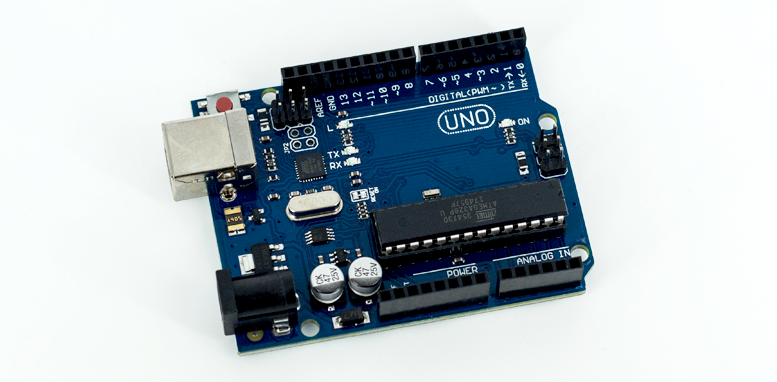
\includegraphics[width = 0.8\textwidth]{Caps/Figs/mat-met/arduino.png}
   \label{fig:arduino-uno}
    \fonte{Site\protect\footnotemark}
\end{figure}
\footnotetext{Disponível em: \url{https://uploads.filipeflop.com/2014/09/01.png}. Acesso em: 8 set. 2020.}

Para o software será utilizado o ambiente de desenvolvimento integrado (IDE - \textit{Integrated Development Environment}) disponibilizado pelo próprio arduino para download em seu site oficial.

\nomenclature{IDE}{\textit{Integrated Development Environment}}
\nomenclature{USB}{\textit{Universal Serial Bus}}

%================================================================================
\section{Raspberry Pi}
\label{sec:raspberrypi}

Raspberry Pi é um computador de placa única de tamanho reduzido que se conecta com periféricos.

%================================================================================

\section{Robo Móvel}
\label{sec:robomovel}

%================================================================================

\section{Sensores}
\label{sec:sensores}


%================================================================================








